\chapter{Antarmuka, Surfaktan, dan Koloid}\label{ch:b3:colloids}

Mayones adalah minyak yang terdispersi sebagai tetesan berukuran beberapa
mikrometer di dalam sedikit air dan cuka, yang dijaga tetap terpisah oleh
lesitin dan protein kuning telur. Jika dikocok terlalu cepat pada awalnya, atau
jika minyaknya dituang terlalu cepat, mayones itu pecah menjadi lapisan
berminyak dan lapisan berair: tetesan-tetesannya bergabung, dan energi yang
menjaganya tetap terpisah pun hilang. Susu, kabut, tinta, cat, darah, dan air
sungai yang keruh adalah materi sejenis, yaitu partikel atau tetesan yang jauh
lebih besar daripada molekul dan jauh lebih kecil daripada apa pun yang dapat
dilihat mata, begitu banyak sehingga sebagian besar molekulnya berada dekat
dengan sebuah antarmuka. Bab ini membahas energi antarmuka, molekul-molekul
yang menurunkannya, \omterm{def:b3:colloids:colloid}{koloid} yang dimungkinkan oleh antarmuka, dan apa yang
menjaga \omterm{def:b3:colloids:colloid}{koloid} tetap terdispersi atau membuatnya berkoagulasi.

\begin{recall}
Jilid Tahun 1 menyebut amfifilik molekul yang memiliki kepala hidrofilik dan
ekor hidrofobik, serta menjelaskan interaksi London dan permitivitas relatif
pelarut; bagian Kelas 11 jilid pertama memperkenalkan \omterm{def:b3:colloids:micelle}{misel} dalam sabun. Jilid
Tahun 2 mendefinisikan potensial kimia, kekuatan ion, dan aktivitas.
\Cref{ch:b3:surfaces-catalysis} membahas \omterm{def:b3:surfaces-catalysis:adsorption}{adsorpsi} pada padatan,
\cref{ch:b3:electrode-kinetics} \omterm{def:b3:electrode-kinetics:double-layer}{lapisan rangkap listrik} dan \omterm{def:b3:electrode-kinetics:double-layer}{panjang Debye-nya}.
Dari fisika: gerak Brown, dan tekanan di dalam permukaan yang melengkung.
\end{recall}

\begin{omfigure}
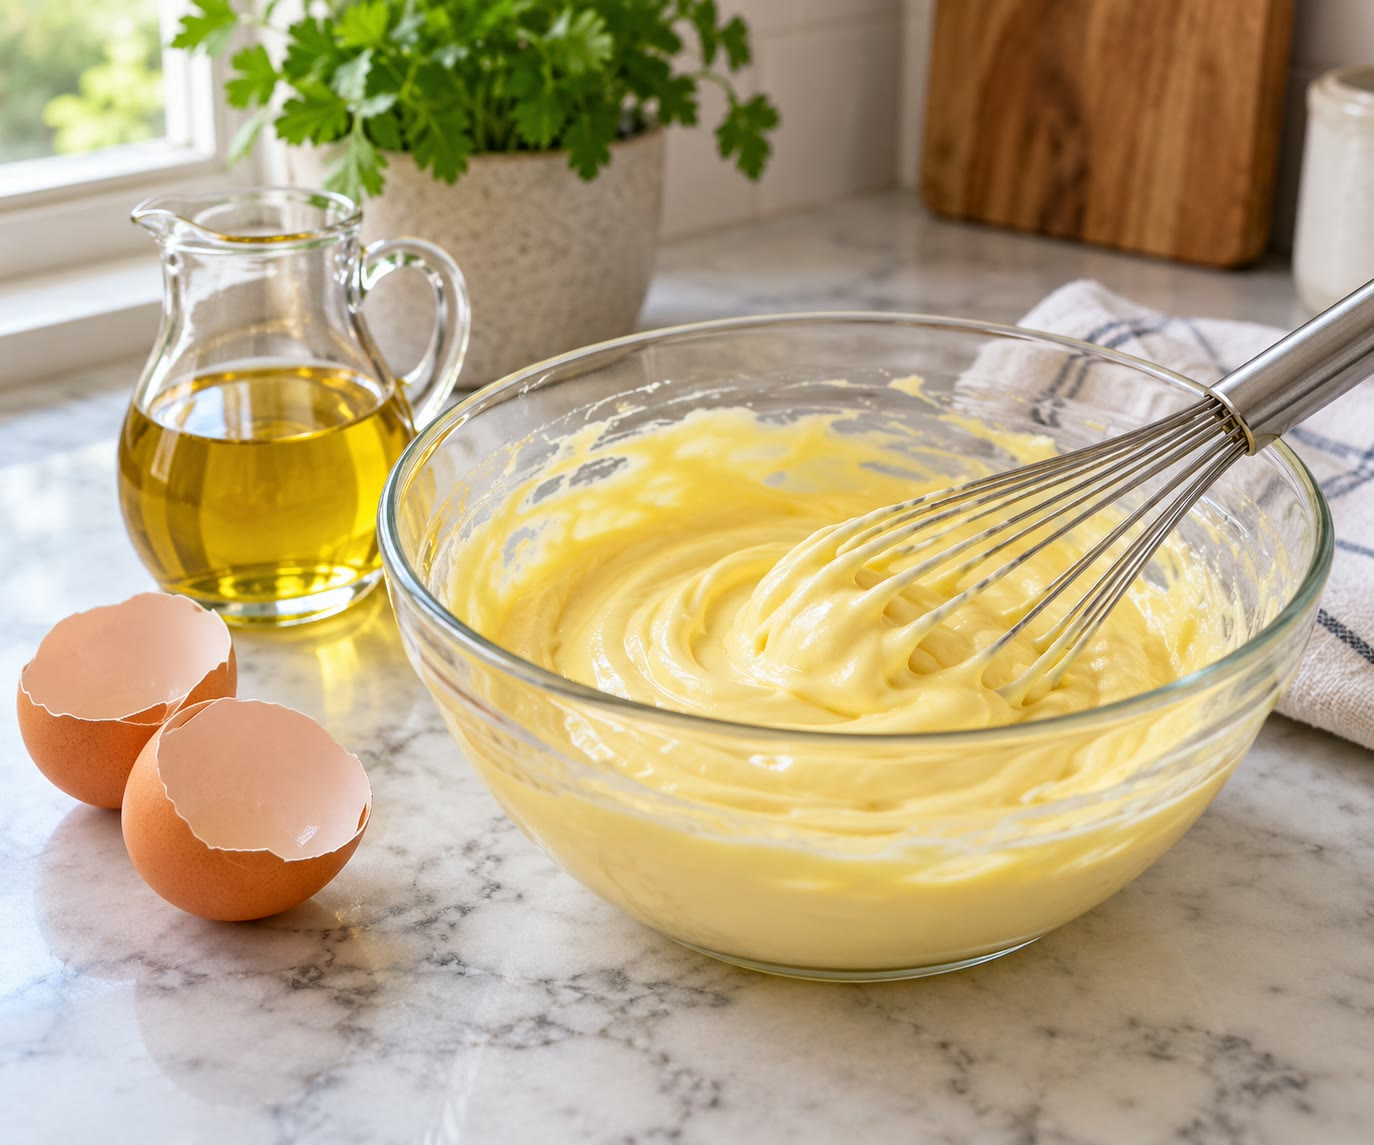
\includegraphics[width=0.6\linewidth]{images/book4/ai/b3-17-mayonnaise.jpg}

{\small Mayones yang sedang dikocok: \omterm{def:b3:colloids:colloid}{emulsi} tetesan minyak dalam air, yang
distabilkan oleh \omterm{def:b3:colloids:surfactant}{surfaktan} kuning telur.}
\end{omfigure}

\section{Antarmuka dan tegangan permukaan}

Molekul di bagian dalam cairan ditarik sama kuat ke segala arah; di permukaan,
molekul itu kehilangan sebagian tetangganya. Membuat permukaan memerlukan energi.

\begin{definition}[Tegangan permukaan]\label{def:b3:colloids:surface-tension}
Yang disebut \emph{tegangan permukaan}\index{tegangan permukaan} $\gamma$ sebuah cairan adalah energi
Gibbs yang diperlukan untuk membuat satu satuan luas permukaannya pada suhu,
tekanan, dan komposisi tetap: $\gamma = (\partial G/\partial A)_{T,p,n}$, dalam \unit{J.m^{-2}} $=$ \unit{N.m^{-1}}. Untuk
antarmuka antara dua fase, besaran ini disebut tegangan antarmuka.
\end{definition}

Air, yang disatukan oleh ikatan hidrogen, memiliki \omterm{def:b3:colloids:surface-tension}{tegangan permukaan} yang tinggi: \qty{72.0}{mN/m}
pada \qty{25}{\celsius}. Alkana sekitar 20, raksa sekitar 480.

\begin{proposition}[Tekanan Laplace]\label{prop:b3:colloids:laplace}
Tekanan di dalam tetes atau gelembung bulat berjari-jari $r$ melebihi tekanan
di luarnya sebesar
\[
  \Delta p = \frac{2\gamma}{r} .
\]
\end{proposition}

\begin{proof}
Perbesarlah jari-jarinya sebesar $\dd r$ pada kesetimbangan: kerja yang dilakukan oleh selisih
tekanan, $\Delta p\,4\pi r^2\dd r$, sama dengan pertambahan energi Gibbs permukaan, $\gamma\,8\pi r\,\dd r$.
\end{proof}

\begin{definition}[Sudut kontak, pembasahan]\label{def:b3:colloids:wetting}
Yang disebut \emph{sudut kontak}\index{sudut kontak} $\theta$ sebuah tetes pada padatan adalah sudut,
yang diukur melalui cairan, antara permukaan padatan dan permukaan cairan
pada garis tempat padatan, cairan, dan uap bertemu. Sebuah cairan
\emph{membasahi}\index{pembasahan} padatan jika $\theta < 90^\circ$, dan menyebar sepenuhnya jika $\theta = 0$.
\end{definition}

\begin{theorem}[Persamaan Young]\label{thm:b3:colloids:young}
Pada kesetimbangan, ketiga tegangan antarmuka dan \omterm{def:b3:colloids:wetting}{sudut kontak} memenuhi
\[
  \gamma_{\mathrm{SV}} = \gamma_{\mathrm{SL}} + \gamma_{\mathrm{LV}}\cos\theta .
\]
Inilah \emph{persamaan Young}\index{persamaan Young}.
\end{theorem}

\begin{proof}
Geserlah garis kontak ke luar sejauh $\dd x$ (per satuan panjang garis): antarmuka padatan--uap
seluas $\dd x$ digantikan oleh antarmuka padatan--cairan, dan antarmuka
cairan--uap bertambah sebesar $\dd x\cos\theta$. Energi Gibbs berubah sebesar
$(\gamma_{\mathrm{SL}} - \gamma_{\mathrm{SV}} + \gamma_{\mathrm{LV}}\cos\theta)\dd x$, yang bernilai nol pada kesetimbangan.
\end{proof}

\begin{omfigure}
\begin{tikzpicture}[font=\small, >=Stealth]
  \fill[black!12] (-3.6,-0.5) rectangle (3.6,0);
  \draw[thick] (-3.6,0) -- (3.6,0);
  \node[anchor=north] at (2.6,-0.05) {padatan};
  \fill[omWater!60] (-2.0,0) arc[start angle=160, end angle=20, radius=2.13] -- cycle;
  \draw[thick, omDef] (-2.0,0) arc[start angle=160, end angle=20, radius=2.13];
  % pusat lingkaran 0.73 di bawah padatan: tudung yang lebih kecil daripada setengah bola, sudut kontak 90 - 20 = 70 derajat;
  % di titik kontak kanan, permukaan cairan meninggalkannya pada 110 derajat (ke atas dan ke kiri)
  \draw[->, thick, omThm] (2.0,0) -- ++(110:1.3) node[anchor=south] {$\gamma_{\mathrm{LV}}$};
  \draw[->, thick] (2.0,0) -- (3.3,0) node[anchor=south] {$\gamma_{\mathrm{SV}}$};
  \draw[->, thick] (2.0,0) -- (0.7,0) node[anchor=north, yshift=-1pt] {$\gamma_{\mathrm{SL}}$};
  \draw (1.45,0) arc[start angle=180, end angle=110, radius=0.55];
  \node at (1.33,0.42) {$\theta$};
  \node at (0,0.6) {cairan};
  \node at (-2.8,1.4) {uap};
\end{tikzpicture}

{\small Sebuah tetes duduk dan ketiga tegangan yang menarik garis kontaknya:
neraca komponen-komponennya sepanjang padatan memberikan \omterm{thm:b3:colloids:young}{persamaan Young}; di
sini $\theta
\approx 70^\circ$, cairan yang \omterm{def:b3:colloids:wetting}{membasahi} sebagian.}
\end{omfigure}

\begin{theorem}[Persamaan Kelvin]\label{thm:b3:colloids:kelvin}
Tekanan uap sebuah tetes bulat berjari-jari $r$ melebihi tekanan uap cairan
yang permukaannya datar, $p^*$:
\[
  \ln\frac{p}{p^*} = \frac{2\gamma V_{\mathrm m}}{rRT},
\]
dengan $V_{\mathrm m}$ volume molar cairan. Inilah \emph{persamaan
Kelvin}\index{persamaan Kelvin}.
\end{theorem}

\begin{proof}
Cairan di dalam tetes berada di bawah tekanan tambahan $2\gamma/r$, yang menaikkan
potensial kimianya sebesar $V_{\mathrm m}\,2\gamma/r$ (dengan $(\partial\mu/\partial p)_T = V_{\mathrm m}$, cairan dianggap tak termampatkan).
Uap yang berada dalam kesetimbangan dengannya harus mengalami kenaikan
potensial kimia yang sama: $RT\ln(p/p^*) = 2\gamma V_{\mathrm m}/r$.
\end{proof}

Untuk tetesan air berjari-jari \qty{10}{nm} pada \qty{25}{\celsius}, $2\gamma V_{\mathrm m}/rRT = 0.105$: tekanan
uapnya 11\,\% di atas tekanan uap air yang datar. Tetesan kecil menguap
sementara tetesan besar tumbuh, dan awan memerlukan inti untuk mulai
terbentuk; hal yang sama berlaku untuk kelarutan kristal-kristal kecil.

\begin{definition}[Pematangan Ostwald]\label{def:b3:colloids:ripening}
Yang disebut \emph{pematangan Ostwald}\index{pematangan Ostwald} adalah pertumbuhan
partikel atau tetesan yang lebih besar dalam sebuah dispersi dengan
mengorbankan yang lebih kecil, yang didorong oleh kelarutan atau tekanan uap
partikel kecil yang lebih tinggi.
\end{definition}

\section{Surfaktan dan misel}

\begin{definition}[Surfaktan]\label{def:b3:colloids:surfactant}
Yang disebut \emph{surfaktan}\index{surfaktan} (zat aktif permukaan) adalah molekul amfifilik
yang teradsorpsi pada antarmuka dan menurunkan tegangannya. Surfaktan itu
disebut \emph{surfaktan anionik}\index{surfaktan anionik} jika kepalanya berupa
anion (natrium dodesil sulfat, sabun), \emph{surfaktan kationik}\index{surfaktan kationik}
jika berupa kation (garam amonium kuaterner), dan \emph{surfaktan
nonionik}\index{surfaktan nonionik} jika kepalanya berupa gugus polar yang netral
(rantai satuan etilena oksida).
\end{definition}

\begin{definition}[Konsentrasi ekses permukaan]\label{def:b3:colloids:surface-excess}
Yang disebut \emph{konsentrasi ekses permukaan}\index{konsentrasi ekses permukaan} $\Gamma$ sebuah
zat terlarut adalah jumlah zat terlarut pada antarmuka per satuan luas, yang
melebihi jumlah yang akan dimuat oleh volume yang sama seandainya konsentrasi
di bagian dalam larutan berlaku sampai tepat di antarmuka.
\end{definition}

\begin{theorem}[Isoterm adsorpsi Gibbs]\label{thm:b3:colloids:gibbs-adsorption}
Untuk larutan encer zat terlarut nonionik berkonsentrasi $c$,
\[
  \Gamma = -\frac{1}{RT}\frac{\dd\gamma}{\dd\ln c};
\]
untuk \omterm{def:b3:colloids:surfactant}{surfaktan} ionik 1:1 tanpa garam tambahan, $RT$ diganti dengan $2RT$. Inilah
\emph{isoterm adsorpsi Gibbs}\index{isoterm adsorpsi Gibbs}.
\end{theorem}

\begin{proof}
Untuk antarmuka, padanan hubungan Gibbs--Duhem pada $T$ dan
$p$ tetap adalah $\dd\gamma = -\sum_i\Gamma_i\,\dd\mu_i$ (energi Gibbs permukaan $\gamma A$ berperan sebagai $G$,
diterima tanpa bukti). Dengan memilih permukaan pembagi sedemikian rupa sehingga pelarut tidak memiliki ekses,
$\dd\gamma = -\Gamma\,\dd\mu$, dan dalam larutan encer $\dd\mu = RT\,\dd\ln c$. Untuk \omterm{def:b3:colloids:surfactant}{surfaktan} ionik,
kation dan anionnya sama-sama teradsorpsi dengan ekses yang sama dan $\dd\mu$ menjadi
$2RT\,\dd\ln c$.
\end{proof}

\omterm{def:b3:colloids:surfactant}{Surfaktan} yang \omterm{def:b3:colloids:surface-tension}{tegangan permukaannya} menurun secara linear terhadap $\ln c$ memiliki ekses
permukaan yang tetap: antarmukanya jenuh, dan $1/(\Gamma N_A)$ adalah luas yang ditempati oleh
satu molekul yang teradsorpsi.

\begin{method}[Luas per molekul dari kemiringan $\gamma$--$\ln c$]\label{met:b3:colloids:surface-excess}
\begin{enumerate}
  \item Ukurlah $\gamma$ terhadap $c$ di bawah CMC; alurkan $\gamma$ terhadap $\ln c$.
  \item Ambillah kemiringan bagian linear tepat di bawah CMC; $\Gamma = -\text{kemiringan}/(nRT)$, $n
        = 1$ untuk \omterm{def:b3:colloids:surfactant}{surfaktan nonionik}, 2 untuk \omterm{def:b3:colloids:surfactant}{surfaktan} ionik 1:1 tanpa garam.
  \item Luas per molekul $= 1/(\Gamma N_A)$; nilai-nilai khasnya 0.3 sampai \qty{0.6}{nm^2}.
\end{enumerate}
\end{method}

\begin{definition}[Misel, konsentrasi misel kritis, bilangan agregasi]\label{def:b3:colloids:micelle}
Yang disebut \emph{misel}\index{misel} adalah agregat molekul \omterm{def:b3:colloids:surfactant}{surfaktan} dalam larutan
yang ekor-ekor hidrofobiknya membentuk inti mirip cairan yang dilindungi dari air oleh
kepala-kepalanya. Yang disebut \emph{konsentrasi misel kritis}\index{konsentrasi misel kritis}
(CMC) adalah konsentrasi yang di atasnya misel terbentuk; jumlah
rata-rata molekul dalam misel disebut \emph{bilangan agregasi}\index{bilangan agregasi}.
\end{definition}

\begin{proposition}[Patahan pada CMC]\label{prop:b3:colloids:cmc-break}
Di atas CMC, konsentrasi \omterm{def:b3:colloids:surfactant}{surfaktan} bebas, dan bersamanya \omterm{def:b3:colloids:surface-tension}{tegangan permukaan}
dan tekanan osmotik, hampir tetap; sifat-sifat yang bergantung pada
molekul bebas berubah kemiringannya pada CMC.
\end{proposition}

\begin{proof}[Bukti parsial]
Perlakukan \omterm{def:b3:colloids:micelle}{misel} sebagai fase tersendiri: \omterm{def:b3:colloids:surfactant}{surfaktan} yang ditambahkan masuk ke dalam \omterm{def:b3:colloids:micelle}{misel} begitu
potensial kimia molekul bebas mencapai potensial kimia sebuah molekul dalam
\omterm{def:b3:colloids:micelle}{misel}, dan potensial kimia ini, jadi juga konsentrasi bebasnya, sesudah itu tetap.
\omterm{def:b3:colloids:surface-tension}{Tegangan permukaan}, yang ditentukan oleh molekul bebas melalui isoterm
Gibbs, berhenti menurun; konduktivitas tetap naik, tetapi lebih lambat, karena
\omterm{def:b3:colloids:micelle}{misel} membawa muatan per \omterm{def:b3:colloids:surfactant}{surfaktan} yang lebih kecil daripada ion bebas (sebagian
ion pengimbangnya terikat). Model ini merupakan sebuah limit, karena \omterm{def:b3:colloids:micelle}{misel} yang
ukurannya terhingga terbentuk dalam rentang konsentrasi yang sempit (diterima
tanpa bukti).
\end{proof}

\begin{method}[CMC dari sebuah patahan]\label{met:b3:colloids:cmc}
\begin{enumerate}
  \item Ukurlah \omterm{def:b3:colloids:surface-tension}{tegangan permukaan} (atau, untuk \omterm{def:b3:colloids:surfactant}{surfaktan} ionik,
        konduktivitas) dalam rentang konsentrasi yang mencakup CMC yang
        diharapkan.
  \item Cocokkan garis-garis lurus pada kedua cabangnya ($\gamma$ terhadap $\log c$, atau $\kappa$ terhadap $c$).
  \item Titik potong keduanya adalah CMC.
\end{enumerate}
\end{method}

\begin{omfigure}
\begin{tikzpicture}
\begin{axis}[name=gm, width=0.47\linewidth, height=5.2cm, xmin=-5, xmax=-1.5, ymin=30, ymax=76,
  axis lines=left, xlabel={$\log(c/\unit{mol.L^{-1}})$}, ylabel={$\gamma$ / \unit{mN.m^{-1}}},
  tick label style={font=\small}, label style={font=\small}]
\addplot[omDef, very thick] table[x=logc, y=gamma_mN] {figdata/out/bachelor-3-surfactant-cmc-gamma.dat};
\draw[black!40, dashed] (axis cs:-2.086,30) -- (axis cs:-2.086,70);
\node[font=\scriptsize, anchor=south west] at (axis cs:-2.05,45) {CMC};
\end{axis}
\begin{axis}[at={(gm.east)}, anchor=west, xshift=1.4cm, width=0.47\linewidth, height=5.2cm,
  xmin=0, xmax=20, ymin=0, ymax=1.0, axis lines=left, xlabel={$c$ / mM},
  ylabel={$\kappa$ / \unit{mS.cm^{-1}}}, tick label style={font=\small}, label style={font=\small}]
\addplot[omThm, very thick] table[x=c_mM, y=kappa] {figdata/out/bachelor-3-surfactant-cmc-kappa.dat};
\draw[black!40, dashed] (axis cs:8.2,0) -- (axis cs:8.2,0.9);
\node[font=\scriptsize, anchor=south west] at (axis cs:8.4,0.15) {CMC};
\end{axis}
\end{tikzpicture}

{\small Sebuah \omterm{def:b3:colloids:surfactant}{surfaktan} ionik model dengan CMC natrium dodesil sulfat,
\qty{8.2}{mM} pada \qty{25}{\celsius}. Kiri: \omterm{def:b3:colloids:surface-tension}{tegangan permukaan} menurun terhadap $\log c$, secara linear tepat di bawah
CMC (antarmuka yang jenuh, luas sekitar \qty{0.6}{nm^2} per molekul), lalu tetap.
Kanan: konduktivitas naik dengan lebih landai di atas CMC.}
\end{omfigure}

\begin{definition}[Parameter kemasan]\label{def:b3:colloids:packing}
Yang disebut \emph{parameter kemasan}\index{parameter kemasan} sebuah \omterm{def:b3:colloids:surfactant}{surfaktan} adalah $P =
v/(a_0l)$, dengan $v$ volume ekor hidrofobiknya, $l$ panjang ekor yang terentang,
dan $a_0$ luas optimal per gugus kepala di permukaan agregat.
\end{definition}

\begin{proposition}[Bentuk agregat]\label{prop:b3:colloids:packing}
\omterm{def:b3:colloids:micelle}{Misel} bulat memerlukan $P \le \frac13$, \omterm{def:b3:colloids:micelle}{misel} silinder $\frac13 < P \le \frac12$, dan lapisan ganda datar
(vesikel, membran) $\frac12 < P \le 1$; $P > 1$ memberikan struktur terbalik.
\end{proposition}

\begin{proof}
Dalam sebuah bola berjari-jari $R \le l$ yang tersusun dari $N$ molekul, $Nv = \frac43\pi R^3$ dan $Na_0 = 4\pi R^2$, sehingga
$v/a_0 = R/3 \le l/3$: $P \le \frac13$. Untuk silinder berjari-jari $R$ dan panjang $L$, $Nv = \pi R^2L$ dan
$Na_0 = 2\pi RL$: $v/a_0 = R/2 \le l/2$. Untuk lapisan ganda setebal $2l$ dan seluas $A$, $Nv = 2lA$ dan
$Na_0 = 2A$: $v/a_0 = l$.
\end{proof}

\begin{omfigure}
\begin{tikzpicture}[font=\scriptsize]
  % kerucut pembentuk bola
  \draw[omDef, thick, fill=omDef!15] (0,0) -- (-0.45,1.2) arc[start angle=180, end angle=0, radius=0.45] -- cycle;
  \node at (0,-0.3) {$P < \frac13$: kerucut};
  % misel
  \begin{scope}[xshift=2.2cm, yshift=0.6cm]
    \foreach \a in {0,30,...,330}{\draw[black!60] (\a:0.2) -- (\a:0.62); \fill[omDef] (\a:0.7) circle (0.09);}
    \node at (0,-1.05) {misel bulat};
  \end{scope}
  % kerucut terpancung
  \begin{scope}[xshift=4.7cm]
    \draw[omDef, thick, fill=omDef!15] (-0.18,0) -- (-0.4,1.2) -- (0.4,1.2) -- (0.18,0) -- cycle;
    \node at (0,-0.3) {$\frac13 < P < \frac12$};
  \end{scope}
  \begin{scope}[xshift=6.9cm, yshift=0.6cm]
    \fill[omDef!10] (-0.9,-0.55) rectangle (0.9,0.55);
    \foreach \x in {-0.8,-0.5,...,0.8}{\fill[omDef] (\x,0.62) circle (0.08); \fill[omDef] (\x,-0.62) circle (0.08);}
    \node[align=center] at (0,-1.15) {silinder\\ (tampak samping)};
  \end{scope}
  % bentuk silinder
  \begin{scope}[xshift=9.4cm]
    \draw[omDef, thick, fill=omDef!15] (-0.3,0) rectangle (0.3,1.2);
    \node at (0,-0.3) {$P \approx 1$: silinder};
  \end{scope}
  \begin{scope}[xshift=11.4cm, yshift=0.6cm]
    \foreach \x in {-0.8,-0.6,...,0.8}{
      \draw[black!60] (\x,0.5) -- (\x,0.05) (\x,-0.5) -- (\x,-0.05);
      \fill[omDef] (\x,0.58) circle (0.08); \fill[omDef] (\x,-0.58) circle (0.08);}
    \node at (0,-1.05) {lapisan ganda};
  \end{scope}
\end{tikzpicture}

{\small Bentuk molekul dan bentuk agregat. \omterm{def:b3:colloids:surfactant}{Surfaktan} dengan kepala yang besar
dan satu ekor (sebuah kerucut) tersusun menjadi \omterm{def:b3:colloids:micelle}{misel} bulat; dengan kepala
yang lebih kecil, menjadi silinder; molekul yang ekornya selebar kepalanya,
seperti lipid berantai dua, menjadi lapisan ganda datar, yaitu dinding vesikel
dan membran sel.}
\end{omfigure}

Daya deterjen memadukan efek-efek ini: \omterm{def:b3:colloids:surfactant}{surfaktan} menurunkan tegangan antarmuka
antara air dan kotoran berminyak sampai kotoran itu menggulung menjadi
tetes-tetes, yang kemudian dilarutkan oleh \omterm{def:b3:colloids:micelle}{misel} di dalam intinya.

\section{Koloid}

\begin{definition}[Koloid]\label{def:b3:colloids:colloid}
Yang disebut \emph{koloid}\index{koloid} adalah dispersi partikel, tetesan, atau gelembung
yang berukuran kira-kira \qty{1}{nm} sampai \qty{1}{\micro m} (yaitu \emph{fase terdispersi}\index{fase terdispersi})
di dalam \emph{medium pendispersi}\index{medium pendispersi} yang kontinu. Yang disebut
\emph{sol}\index{sol} adalah dispersi partikel padat dalam cairan,
\emph{emulsi}\index{emulsi} adalah dispersi tetesan cairan dalam cairan lain,
\emph{busa}\index{busa} adalah dispersi gelembung gas dalam cairan atau padatan,
\emph{gel}\index{gel} adalah jaringan partikel atau polimer yang merentang di
seluruh cairan dan membuatnya mirip padatan, dan \emph{aerosol}\index{aerosol}
adalah dispersi tetesan atau partikel dalam gas.
\end{definition}

Partikel \omterm{def:b3:colloids:colloid}{koloid} cukup kecil untuk tetap melayang karena gerak Brown (tumbukan
acak molekul-molekul pelarut, dari fisika) dan cukup besar untuk menghamburkan
cahaya.

\begin{definition}[Efek Tyndall]\label{def:b3:colloids:tyndall}
Yang disebut \emph{efek Tyndall}\index{efek Tyndall} adalah penghamburan cahaya oleh
partikel-partikel \omterm{def:b3:colloids:colloid}{koloid}, yang membuat berkas cahaya tampak dari samping ketika
melintasi \omterm{def:b3:colloids:colloid}{koloid} itu, sedangkan larutan sejati tetap tidak tampak.
\end{definition}

\begin{omfigure}
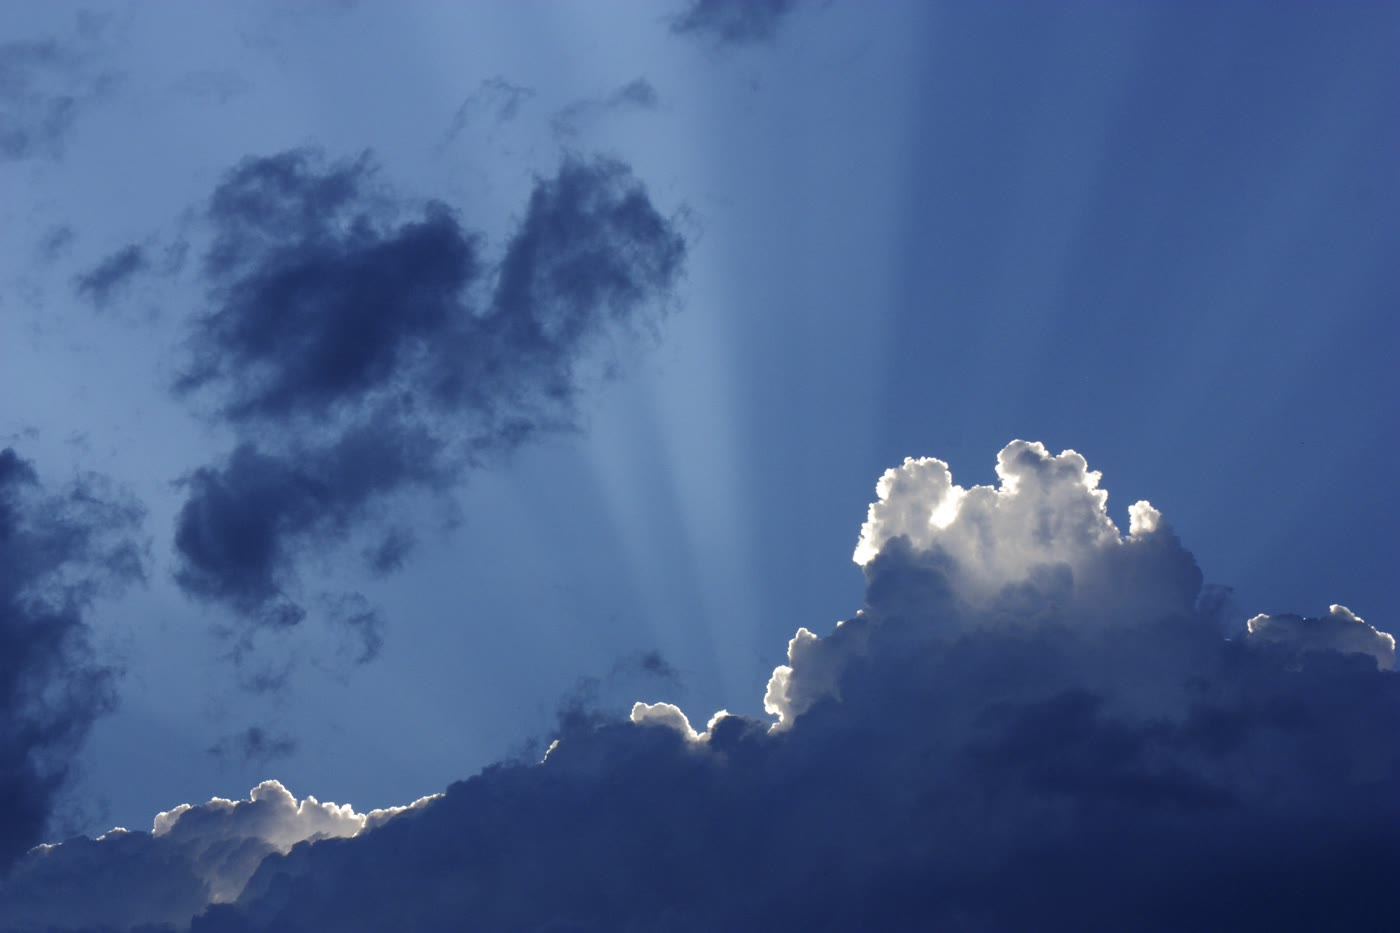
\includegraphics[width=0.55\linewidth]{images/book4/tyndall-sky.jpg}

{\small Berkas sinar matahari yang menembus celah awan: berkas itu tampak karena
\omterm{def:b3:colloids:colloid}{aerosol} udara, yaitu tetesan dan debu, menghamburkan sebagian cahaya ke
samping; inilah \omterm{def:b3:colloids:tyndall}{efek Tyndall} dalam skala langit.}
\end{omfigure}

\section{Kestabilan koloid}

Dua partikel \omterm{def:b3:colloids:colloid}{koloid} selalu saling menarik pada jarak pendek oleh gaya van der
Waals. Di dalam air, sebagian besar partikel juga bermuatan (gugus permukaan
yang terionisasi, ion yang teradsorpsi), dan dikelilingi oleh \omterm{def:b3:electrode-kinetics:double-layer}{lapisan difus}
ion pengimbang, yaitu lapisan rangkap pada \cref{ch:b3:electrode-kinetics}. Ketika
dua partikel saling mendekat, lapisan-lapisan difusnya bertumpang tindih dan
saling menolak.

\begin{definition}[Potensial zeta]\label{def:b3:colloids:zeta}
Yang disebut \emph{potensial zeta}\index{potensial zeta} $\zeta$ sebuah partikel adalah potensial
listrik pada bidang gelincirnya, yaitu batas di dalam lapisan rangkap antara
cairan yang bergerak bersama partikel dan cairan yang tidak; potensial ini
diukur dari kecepatan partikel dalam medan listrik (elektroforesis).
\end{definition}

\begin{omfigure}
\begin{tikzpicture}[font=\scriptsize]
  \fill[black!20] (0,0) circle (1.2);
  \foreach \a in {0,30,...,330}{\node at (\a:1.05) {$-$};}
  \draw[omDef, dashed] (0,0) circle (1.55);
  \foreach \a in {15,45,...,345}{\draw[omDef, fill=omDef!15] (\a:1.38) circle (0.11); \node at (\a:1.38) {\tiny$+$};}
  \draw[omThm, thick, densely dotted] (0,0) circle (1.85);
  \foreach \a/\r/\s in {10/2.2/+, 50/2.5/+, 95/2.3/-, 130/2.7/+, 175/2.2/+, 215/2.6/-, 250/2.3/+, 290/2.8/+, 345/2.6/+}{
    \draw[black!60, fill=white] (\a:\r) circle (0.11); \node at (\a:\r) {\tiny$\s$};}
  \draw[->, black!60] (2.6,1.6) node[anchor=west] {lapisan Stern} -- (40:1.6);
  \draw[->, omThm] (2.6,-1.4) node[anchor=west] {bidang gelincir: $\zeta$} -- (-30:1.87);
  \node at (0,0) {partikel};
  \node[anchor=west] at (2.9,0.2) {lapisan difus};
\end{tikzpicture}

{\small Partikel bermuatan negatif dengan lapisan rangkapnya: lapisan Stern
yang kompak berisi ion pengimbang, bidang gelincir tepat di luarnya, tempat
\omterm{def:b3:colloids:zeta}{potensial zeta} didefinisikan, dan \omterm{def:b3:electrode-kinetics:double-layer}{lapisan difus}, tempat ion pengimbang lebih
banyak daripada ion sejenis dalam rentang beberapa \omterm{def:b3:electrode-kinetics:double-layer}{panjang Debye}.}
\end{omfigure}

\begin{theorem}[Teori DLVO]\label{thm:b3:colloids:dlvo}
Untuk dua bola berjari-jari $a$ yang dipisahkan oleh celah $h \ll a$, dengan potensial \omterm{def:b3:electrode-kinetics:double-layer}{lapisan difus}
$\psi$ dan tetapan Hamaker $A$, energi interaksinya, untuk potensial yang rendah, adalah
\[
  V(h) = 2\pi\varepsilon_r\varepsilon_0a\psi^2\ln\bigl(1 + \eu^{-\kappa h}\bigr) - \frac{Aa}{12h} .
\]
Suku pertama, yaitu tolakan lapisan rangkap, meluruh dalam jarak sepanjang \omterm{def:b3:electrode-kinetics:double-layer}{panjang Debye} $\kappa^{-1}$;
suku kedua, yaitu tarikan van der Waals, tidak bergantung pada garam. Jumlah keduanya
memiliki penghalang energi pada jarak beberapa \omterm{def:b3:electrode-kinetics:double-layer}{panjang Debye} ketika konsentrasi
garamnya rendah, dan tidak memilikinya di atas sebuah konsentrasi kritis.
\end{theorem}

\begin{proof}[Bukti parsial]
Kedua bentuk itu diterima tanpa bukti (tolakan dari tumpang tindih dua lapisan
Gouy--Chapman dalam pendekatan Derjaguin, tarikan dari penjumlahan interaksi
London atas kedua benda). Menaikkan kekuatan ion menaikkan $\kappa$
(\cref{prop:b3:electrode-kinetics:debye-length}): tolakan lalu lenyap pada
$h$ yang lebih kecil, tempat tarikan, yang tumbuh sebagai $1/h$, lebih kuat; maksimum
$V$ berkurang dan akhirnya lenyap.
\end{proof}

\begin{omfigure}
\begin{tikzpicture}
\begin{axis}[width=0.72\linewidth, height=5.6cm, xmin=0, xmax=30, ymin=-40, ymax=45,
  axis lines=left, xlabel={celah $h$ / nm}, ylabel={$V/kT$},
  tick label style={font=\small}, label style={font=\small},
  legend style={font=\scriptsize, draw=none, at={(0.98,0.98)}, anchor=north east}, legend cell align=left]
\addplot[omDef, thick] table[x=h_nm, y=I1] {figdata/out/bachelor-3-dlvo.dat};
\addplot[black!60, thick] table[x=h_nm, y=I10] {figdata/out/bachelor-3-dlvo.dat};
\addplot[omThm, thick] table[x=h_nm, y=I50] {figdata/out/bachelor-3-dlvo.dat};
\addplot[black, thick, dashed] table[x=h_nm, y=I200] {figdata/out/bachelor-3-dlvo.dat};
\draw[black!30] (axis cs:0,0) -- (axis cs:30,0);
\legend{\qty{1}{mM}, \qty{10}{mM}, \qty{50}{mM}, \qty{200}{mM}}
\end{axis}
\end{tikzpicture}

{\small Interaksi DLVO dua partikel berjari-jari \qty{100}{nm} (model: potensial \omterm{def:b3:electrode-kinetics:double-layer}{lapisan difus}
\qty{-30}{mV}, tetapan Hamaker \qty{2e-20}{J}) dalam air dengan garam 1:1. Pada \qty{1}{mM}
penghalang sekitar $40\,kT$ menjaga partikel-partikel tetap terpisah; pada \qty{10}{mM} penghalang itu tinggal setengahnya;
di dekat \qty{50}{mM} penghalang itu lenyap dan setiap tumbukan menyebabkan pelekatan.}
\end{omfigure}

\begin{definition}[Koagulasi dan stabilisasi]\label{def:b3:colloids:stability}
Yang disebut \emph{koagulasi}\index{koagulasi} adalah agregasi partikel \omterm{def:b3:colloids:colloid}{koloid}
yang disebabkan oleh hilangnya tolakan elektrostatiknya; \emph{flokulasi}\index{flokulasi}
adalah agregasi menjadi flok-flok yang longgar, yang sering dijembatani oleh
polimer yang teradsorpsi. Yang disebut
\emph{konsentrasi koagulasi kritis}\index{konsentrasi koagulasi kritis}
(CCC) sebuah elektrolit adalah konsentrasi yang di atasnya sebuah
\omterm{def:b3:colloids:colloid}{koloid} berkoagulasi dengan cepat. Pada \emph{stabilisasi sterik}\index{stabilisasi sterik},
partikel-partikel dijaga tetap terpisah oleh rantai polimer yang
teradsorpsi atau tercangkok, yang tumpang tindihnya akan mengorbankan entropi.
\end{definition}

\begin{proposition}[Aturan Schulze--Hardy]\label{prop:b3:colloids:schulze-hardy}
Untuk \omterm{def:b3:colloids:colloid}{koloid} yang muatannya tinggi, \omterm{def:b3:colloids:stability}{konsentrasi koagulasi kritis} sebuah
elektrolit berubah sebanding dengan pangkat enam negatif muatan $z$ ion
pengimbangnya: $\text{CCC} \propto z^{-6}$, dengan perbandingan $1 : \frac{1}{64} : \frac{1}{729}$ untuk $z = 1, 2, 3$.
\end{proposition}

\begin{proof}[Bukti parsial]
Tinjaulah dua pelat datar. Pada potensial permukaan yang tinggi, tolakan lapisan rangkap per
satuan luas mendekati $V_R = (64nkT/\kappa)\eu^{-\kappa h}$, dengan $n$ rapat jumlah elektrolit $z{:}z$,
yang tidak bergantung pada potensialnya (diterima tanpa bukti); tarikannya adalah $V_A =
-A/(12\pi h^2)$. Pada CCC, penghalangnya tepat lenyap: $V = 0$ dan $\dd V/\dd h = 0$ pada celah yang
sama. Karena $\dd V_R/\dd h = -\kappa V_R$ dan $\dd V_A/\dd h = -2V_A/h$, kedua syarat itu memberikan
$\kappa V_R = 2V_R/h$, sehingga $\kappa h = 2$, lalu $64nkT\eu^{-2}/\kappa = A\kappa^2/(48\pi)$, yaitu $n \propto \kappa^3$. Dengan
$\kappa^2 = 2nz^2e^2/(\varepsilon kT)$, $\kappa^3 \propto (nz^2)^{3/2}$ dan $n \propto n^{3/2}z^3$: jadi $n \propto z^{-6}$.
\end{proof}

\begin{omfigure}
\begin{tikzpicture}[font=\small, >=Stealth]
  \foreach \x/\lab/\v in {0/\ce{Na+}/1, 2.6/\ce{Ca^{2+}}/{1/64}, 5.2/\ce{Al^{3+}}/{1/729}}{
    \node at (\x,0) {\lab};
    \node[font=\scriptsize] at (\x,-0.45) {CCC $\times\,\v$};}
  \draw[->, thick, omDef] (-0.8,-0.95) -- (6.0,-0.95) node[midway, below, font=\scriptsize] {dosis yang lebih kecil untuk mengoagulasi koloid negatif};
\end{tikzpicture}

{\small Aturan Schulze--Hardy untuk \omterm{def:b3:colloids:colloid}{koloid} bermuatan negatif: \omterm{def:b3:colloids:stability}{konsentrasi
koagulasi kritis} menurun sebanding dengan pangkat enam muatan ion pengimbang.}
\end{omfigure}

Aturan ini menjelaskan mengapa garam aluminium begitu efektif untuk
menjernihkan air, dan mengapa sungai mengendapkan muatan lempungnya di tempat
sungai itu bertemu dengan air asin laut.

\begin{method}[Memilih dosis koagulan]\label{met:b3:colloids:coagulant-dose}
\begin{enumerate}
  \item Ukurlah CCC sebuah elektrolit acuan untuk suspensi itu (uji jar dengan
        dosis yang makin besar, sambil mengamati pengendapannya).
  \item Skalakan nilai itu ke ion pengimbang koagulan dengan aturan Schulze--Hardy.
  \item Konversikan menjadi massa garam per meter kubik dengan rumusnya; tambahkan
        secukupnya untuk hidrolisis dan alkalinitas yang dikonsumsinya.
  \item Hindari dosis berlebih: ion pengimbang yang muatannya tinggi dapat membalik
        tanda muatan partikel dan menstabilkannya kembali.
\end{enumerate}
\end{method}

\section{Koloid dalam praktik}

\begin{definition}[Kesetimbangan hidrofilik--lipofilik]\label{def:b3:colloids:hlb}
Yang disebut \emph{kesetimbangan hidrofilik--lipofilik}\index{kesetimbangan hidrofilik--lipofilik}
(HLB) sebuah \omterm{def:b3:colloids:surfactant}{surfaktan nonionik} adalah, dalam skala Griffin, $20$ kali fraksi
massa bagian hidrofiliknya: nilai yang rendah (3 sampai 6) cocok untuk \omterm{def:b3:colloids:colloid}{emulsi}
air dalam minyak, sedangkan nilai yang tinggi (8 sampai 18) cocok untuk \omterm{def:b3:colloids:colloid}{emulsi}
minyak dalam air dan deterjen.
\end{definition}

\omterm{def:b3:colloids:colloid}{Emulsi} tidak stabil secara termodinamika, karena setiap tetesan membawa energi
antarmuka; pengemulsi membuatnya stabil secara kinetika dengan menurunkan
energi itu dan dengan menambahkan lapisan penolak, bermuatan atau sterik, di
sekeliling setiap tetesan. Mayones adalah \omterm{def:b3:colloids:colloid}{emulsi} minyak dalam air yang
minyaknya begitu banyak (sekitar empat perlima volumenya) sehingga
tetesan-tetesannya saling terhimpit, dan hal itu menjadikannya padatan yang
lunak. \omterm{def:b3:colloids:colloid}{Busa} distabilkan oleh \omterm{def:b3:colloids:surfactant}{surfaktan} yang memperlambat terkurasnya lapisan
cairan di antara gelembung; antibusa, sering berupa minyak silikon, menyebar
pada lapisan-lapisan itu dan memecahkannya. Di instalasi air minum, garam
aluminium atau besi(III) mengoagulasi lempung dan \omterm{def:b3:colloids:colloid}{koloid} organik yang membuat air
sungai keruh; hidroksida yang terbentuk menyapu flok-flok itu ke bawah saat
mengendap. Nanopartikel logam dijaga tetap terdispersi oleh ion sitrat yang
teradsorpsi (elektrostatik) atau oleh rantai polimer yang terikat melalui
tiol (sterik).

\begin{inthelab}[Cincin du Noüy]
Sebuah cincin platina, yang dibersihkan dengan dibakar dalam nyala, digantung
pada neraca dan dicelupkan secara mendatar ke dalam cairan, lalu diangkat
perlahan-lahan. Gaya yang diperlukan untuk menariknya menembus permukaan
melewati sebuah maksimum; gaya itu, dibagi dengan dua kali keliling cincin dan
dikoreksi untuk bentuk meniskus yang terangkat, memberikan \omterm{def:b3:colloids:surface-tension}{tegangan permukaan}.
Pengukuran serangkaian larutan \omterm{def:b3:colloids:surfactant}{surfaktan} dimulai dari larutan yang paling
encer, dan cincin dibilas di antara sampel-sampel.
\end{inthelab}

\begin{safety}{\ghs[0.8cm]{GHS02}\ghs[0.8cm]{GHS05}\ghs[0.8cm]{GHS07}}
% ledger: ghs4:SDS, ghs4:Al2SO43
Serbuk natrium dodesil sulfat: padatan mudah menyala, berbahaya jika tertelan,
menyebabkan kerusakan mata yang serius, dan mengiritasi saluran pernapasan;
ditimbang tanpa menerbangkan debu, dengan pelindung mata. Aluminium sulfat
(\ghs[0.6cm]{GHS05}): menyebabkan kerusakan mata yang serius.
\end{safety}

\begin{history}[Tyndall dan ultramikroskop]
Pada 1869 John Tyndall menunjukkan bahwa berkas cahaya menjadi tampak di udara
yang sarat partikel halus dan tidak tampak di udara yang bebas darinya, dan bahwa
cahaya yang terhambur berwarna kebiruan dan terpolarisasi. Richard Zsigmondy,
yang meneliti warna merah \omterm{def:b3:colloids:colloid}{sol} emas, bersama Henry Siedentopf membangun
ultramikroskop pada 1903, yang menyinari \omterm{def:b3:colloids:colloid}{koloid} dari samping dan memperlihatkan
setiap partikel sebagai titik cahaya terhambur di atas latar gelap, terlalu
kecil untuk diuraikan tetapi dapat dihitung. Ia menerima Hadiah Nobel Kimia
1925 untuk karyanya tentang \omterm{def:b3:colloids:colloid}{koloid}.
\end{history}

\section{Latihan}

\begin{exercise}[$\star$]\label{exo:b3:colloids:1}
% ledger: st:H2O.25C
Hitunglah tekanan di dalam gelembung udara berdiameter \qty{1.0}{\micro m} dalam air pada
\qty{25}{\celsius} (di luar: \qty{1.0}{bar}).
\end{exercise}

\begin{exercise}[$\star$]\label{exo:b3:colloids:2}
% ledger: st:H2O.25C
Hitunglah tekanan uap tetesan air berjari-jari \qty{10}{nm} relatif terhadap
air yang datar pada \qty{25}{\celsius} ($V_{\mathrm m} = \qty{18.07}{cm^3/mol}$).
\end{exercise}

\begin{exercise}[$\star$]\label{exo:b3:colloids:3}
Sebuah cairan dengan $\gamma_{\mathrm{LV}} = \qty{72}{mN/m}$ pada padatan dengan $\gamma_{\mathrm{SV}} = \qty{40}{mN/m}$ dan $\gamma_{\mathrm{SL}} =
\qty{20}{mN/m}$ (data latihan): hitunglah \omterm{def:b3:colloids:wetting}{sudut kontaknya}. Apakah cairan itu \omterm{def:b3:colloids:wetting}{membasahi}?
\end{exercise}

\begin{exercise}[$\star$]\label{exo:b3:colloids:4}
% ledger: eps:H2O.25C
Hitunglah \omterm{def:b3:electrode-kinetics:double-layer}{panjang Debye} dalam air pada \qty{25}{\celsius} untuk \qty{0.010}{mol/L} NaCl dan untuk
\ce{MgSO4}.
\end{exercise}

\begin{exercise}[$\star\star$]\label{exo:b3:colloids:5}
Tepat di bawah CMC-nya, \omterm{def:b3:colloids:surface-tension}{tegangan permukaan} sebuah \omterm{def:b3:colloids:surfactant}{surfaktan} ionik (1:1, tanpa garam)
turun \qty{12.6}{mN/m} per satuan $\ln c$ pada \qty{25}{\celsius}. Hitunglah ekses permukaan dan
luas per molekulnya.
\end{exercise}

\begin{exercise}[$\star\star$]\label{exo:b3:colloids:6}
\omterm{def:b3:colloids:surface-tension}{Tegangan permukaan} sebuah \omterm{def:b3:colloids:surfactant}{surfaktan nonionik}: 52.0, 45.5, 39.1, 33.4, 33.3, dan
\qty{33.4}{mN/m} pada $\log c = -5.0$, $-4.5$, $-4.0$, $-3.5$, $-3.0$, dan $-2.5$ (data latihan).
Perkirakan CMC-nya.
\end{exercise}

\begin{exercise}[$\star\star$]\label{exo:b3:colloids:7}
Untuk natrium dodesil sulfat, ambillah $v = \qty{0.350}{nm^3}$, $l = \qty{1.67}{nm}$, dan $a_0 = \qty{0.60}{nm^2}$; untuk
lipid dengan dua rantai semacam itu, $2v$, $l$ yang sama, dan $a_0 = \qty{0.65}{nm^2}$ (data
latihan). Ramalkan bentuk agregat-agregatnya.
\end{exercise}

\begin{exercise}[$\star\star$]\label{exo:b3:colloids:8}
Sebuah \omterm{def:b3:colloids:colloid}{sol} bermuatan negatif berkoagulasi pada \qty{60}{mM} NaCl. Ramalkan CCC dengan \ce{CaCl2}
dan dengan \ce{AlCl3}. Apakah yang akan dilakukan \ce{Na3PO4}?
\end{exercise}

\begin{exercise}[$\star\star$]\label{exo:b3:colloids:9}
% ledger: cmc:C12E6
Hitunglah HLB Griffin heksaetilena glikol monododesil eter,
\ce{C12H25(OCH2CH2)6OH}, yang bagian hidrofiliknya adalah $\ce{(OCH2CH2)6OH}$. Apakah \omterm{def:b3:colloids:surfactant}{surfaktan} itu cocok untuk
\omterm{def:b3:colloids:colloid}{emulsi} minyak dalam air?
\end{exercise}

\begin{exercise}[$\star\star\star$]\label{exo:b3:colloids:10}
Sebuah dispersi mengandung tetesan berjari-jari 50 dan \qty{500}{nm}. Dengan \omterm{thm:b3:colloids:kelvin}{persamaan
Kelvin} yang diterapkan pada kelarutan, jelaskan tetesan mana yang tumbuh dan mana yang menyusut, dan mengapa
\omterm{def:b3:colloids:colloid}{emulsi} makin kasar seiring waktu bahkan tanpa koalesensi.
\end{exercise}

\begin{exercise}[$\star\star\star$]\label{exo:b3:colloids:11}
Tunjukkan dari tekanan Laplace bahwa cairan naik sampai ketinggian $h = 2\gamma\cos\theta/(\rho gr)$ dalam
pipa kapiler berjari-jari $r$, dan hitunglah ketinggian itu untuk air ($\theta = 0$, jari-jari \qty{0.10}{mm}).
\end{exercise}

\begin{exercise}[$\star\star\star$]\label{exo:b3:colloids:12}
Dengan gambar DLVO, jelaskan mengapa penambahan \qty{100}{mM} NaCl pada \omterm{def:b3:colloids:colloid}{sol} yang stabil pada \qty{1}{mM}
membuatnya berkoagulasi, sedangkan penambahan polimer yang tidak teradsorpsi tidak mengubah
penghalangnya, tetapi polimer yang tercangkok pada partikel dapat menjaganya tetap terpisah pada
konsentrasi garam berapa pun.
\end{exercise}

% judul tetap bersama kotak soalnya, yang memenuhi satu halaman sendiri
\clearpage
\enlargethispage{3\baselineskip}
\section{Soal: Menjernihkan Air Keruh dengan Tawas}

\begin{problem}[{Soal akhir pekan --- menjernihkan air keruh dengan tawas:
lapisan rangkap partikel lempung, penghalang DLVO, aturan Schulze--Hardy, dan
dosis aluminium sulfat}]
\label{pb:b3:colloids:1}
% ledger: eps:H2O.25C, visc:H2O.25C
Sebuah instalasi pengolahan air menerima air lunak yang keruh: partikel lempung
berjari-jari \qty{100}{nm} dan berkerapatan \qty{2650}{kg/m^3}, dengan potensial \omterm{def:b3:electrode-kinetics:double-layer}{lapisan difus} \qty{-30}{mV}, dalam
air yang mengandung \qty{1.0}{mM} \ce{NaHCO3}. Uji jar menunjukkan bahwa partikel-partikel itu berkoagulasi
dengan cepat di atas \qty{50}{mM} NaCl (data soal). Instalasi itu mengolah \qty{1000}{m^3} per
jam dengan aluminium sulfat, $\ce{Al2(SO4)3}$ ($M = \qty{342.3}{g/mol}$).

\medskip\noindent\textbf{Bagian I --- \omterm{def:b3:colloids:colloid}{Koloid} yang stabil.}
\begin{enumerate}[beginpenalty=10000]
  \item Mengapa partikel lempung di dalam air bermuatan negatif?
  \item Hitunglah kekuatan ion air itu.
  \item Hitunglah \omterm{def:b3:electrode-kinetics:double-layer}{panjang Debye-nya}.
  \item Bandingkan panjang itu dengan jari-jari partikel. Pendekatan manakah dalam rumus DLVO
        yang dibenarkan oleh hal ini?
  \item Hitunglah kecepatan pengendapan sebuah partikel dengan hukum Stokes, $v =
        2\Delta\rho\,gr^2/9\eta$ ($\eta = \qty{0.89}{mPa.s}$), dalam milimeter per hari.
  \item Mengapa partikel-partikel itu tidak saling melekat ketika bertumbukan?
\end{enumerate}

\medskip\noindent\textbf{Bagian II --- Penghalang DLVO.}
\begin{enumerate}[resume, beginpenalty=10000]
  \item Tuliskan energi DLVO dua partikel.
  \item Bacalah pada gambar tinggi penghalang pada \qty{1}{mM}, dalam satuan $kT$.
  \item Seberapa sering dua partikel yang bertumbukan akan melintasi penghalang semacam itu?
  \item Apakah yang terjadi pada penghalang itu di dekat \qty{50}{mM}?
  \item Jelaskan mengapa penambahan garam menurunkan penghalang itu.
\end{enumerate}

\medskip\noindent\textbf{Bagian III --- Schulze--Hardy.}
\begin{enumerate}[resume, beginpenalty=10000]
  \item Nyatakan aturan itu.
  \item Ramalkan CCC untuk \ce{Ca^{2+}}.
  \item Ramalkan CCC untuk \ce{Al^{3+}}.
  \item Mengapa hanya kation koagulan yang berpengaruh bagi \omterm{def:b3:colloids:colloid}{koloid} ini?
  \item Mengapa sulfat dari tawas hampir tidak berpengaruh pada \omterm{def:b3:colloids:stability}{koagulasi}?
\end{enumerate}

\medskip\noindent\textbf{Bagian IV --- Dosis.}
\begin{enumerate}[resume, beginpenalty=10000]
  \item Hitunglah jumlah \ce{Al^{3+}} yang diperlukan per meter kubik.
  \item Simpulkan jumlah $\ce{Al2(SO4)3}$ per meter kubik.
  \item Simpulkan massanya per meter kubik.
  \item Simpulkan massa yang dipakai instalasi itu per jam.
  \item Di dalam air, \ce{Al^{3+}} terhidrolisis dan bereaksi dengan hidrogenkarbonat. Tuliskan
        persamaan setara yang membentuk \ce{Al(OH)3}.
  \item Berapakah fraksi hidrogenkarbonat yang dikonsumsi oleh dosis itu? Apakah
        pH-nya banyak berubah?
  \item Mengapa dosis berlebih dapat membuat air keruh kembali?
  \item Nyatakan hasilnya: massa minimum aluminium sulfat per meter kubik.
\end{enumerate}
\end{problem}
